Un des principaux buts de l’IoT est de permettre de faciliter un processus dans un environnement donné. En effet, l’automatisation
des tâches et la rapidité établie par les communications via Internet peuvent permettre d’augmenter l’efficacité et la
productivité dans certaines situations. C’est le cas pour le système que nous avons présenté dans les deux précédents rapports, et
que nous continuons d’expliciter dans ce rapport. Le système IoT (Smart Health) dont nous avons la responsabilité de concevoir
permettrait de résoudre le problème de congestion des hôpitaux dans le service des soins intensifs.  
\newline

Dans les deux précédents rapports, nous avons mis en place la conception de notre système dans la couche dispositifs et protocoles
de communication, ou nous avons décrit les différents dispositifs qui pourraient être utilisés dans notre système et comment vont
se dérouler les différentes communications entre les éléments du système, ainsi que dans la couche du middleware, ou nous avons
décrit la couche intergiciel qui s’occupera de gérer le réseau, comme ainsi résumé dans les figures suivantes.  
\newline

Le but de ce rapport est de concevoir la partie application de notre système, ainsi que les services qu’il propose. Nous allons
donc voir comment va se constituer la dernière partie de notre système et quelles sont les différentes fonctionnalités qu’elle va
fournir auprès des différents utilisateurs. Dans les différents dispositifs qui composent notre architecture, nous avons une
multitude de données qui vont transiter dans notre système, toutes ces données vont permettre de faciliter le travail du personnel
médical, avec un la possibilité d’un suivi général du département, mais aussi la possibilité d’avoir un suivi personnalisé et plus
poussé pour un patient. Les données récoltées des différents patients vont pour certaines être partagées avec des hôpitaux
partenaires pour constituer une base de données globale de patients. Et pourront aussi permettre aux proches de la famille d’avoir
accès a certaines informations non sensibles pour se rassurer sur l'état de santé des patients. Il faudra pour cela s’assurer
d’avoir les requis nécessaires dans nos différents services, et pour différents points de vue, à savoir : du point de vue de
l’architecture (c’est-à-dire de notre point de vue), et du points de vue des utilisateurs (le personnel médical, le personnel de
maintenance, l’hôpital, et les proches du patients). La suite de ce rapport sera dédié à une analyse de la qualité de service
(QoS), et de la sécurité et la privacité dans notre système, à savoir à travers les différentes couches de notre système. Quand
nous parlons de QoS, nous faisons référence ici à la disponibilité, et la fiabilité à tous les niveaux de notre système. 

%\begin{figure}[h!]
	%\hspace*{-2.5cm}
	%\centering
	%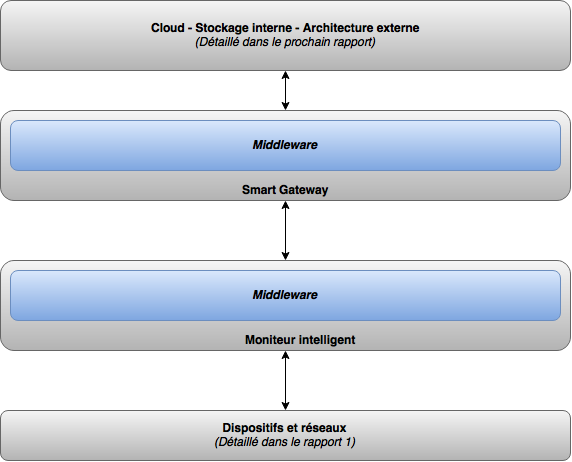
\includegraphics[width=1.4\textwidth]{Figure2.png}
	%\caption{Vue Globale de notre Middleware au sein de notre Système}
	%\label{fig:vueglobale}
%\end{figure}

